% https://northstar-www.dartmouth.edu/doc/idl/html_6.2/Sharpening_an_Image.html
% http://www.dpi.inpe.br/spring/teoria/filtrage/filtragem.htm

Edge + 1, passa alta, agudizaçao, nitidez, "inverso" de blur

\begin{figure}[H]
    \centering
    \begin{kmatrix}
    \matrix(img)[square matrix]{
        -1 & -1 & -1 & -1 & -1 \\
        -1 & 2 & 2 & 2 & -1 \\
        -1 & 2 & 8 & 2 & -1 \\
        -1 & 2 & 2 & 2 & -1 \\
        -1 & -1 & -1 & -1 & -1 \\
    };

    \node[left=of img] {$\displaystyle\Scale[1.7]{\frac{1}{8}}$};
\end{kmatrix}

    \caption{??: $h_{10}$.}
    \label{fig:h10}
\end{figure}

\begin{figure}[H]
    \centering
    \begin{subfigure}{0.48\textwidth}
        \centering
        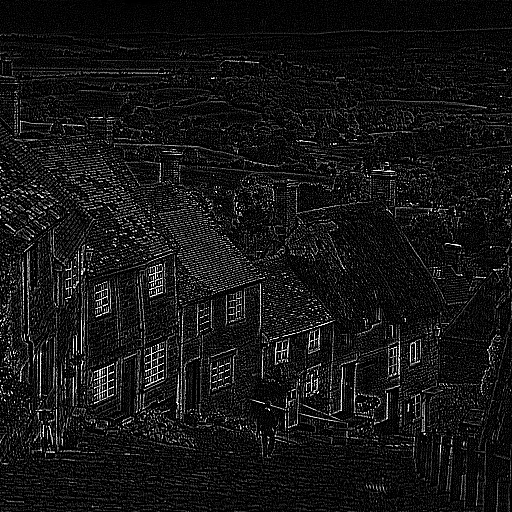
\includegraphics[width=0.9\textwidth]{imagens/city.png}
        \caption{Original: \texttt{city.png}.}
    \end{subfigure}%
    \begin{subfigure}{0.48\textwidth}
        \centering
        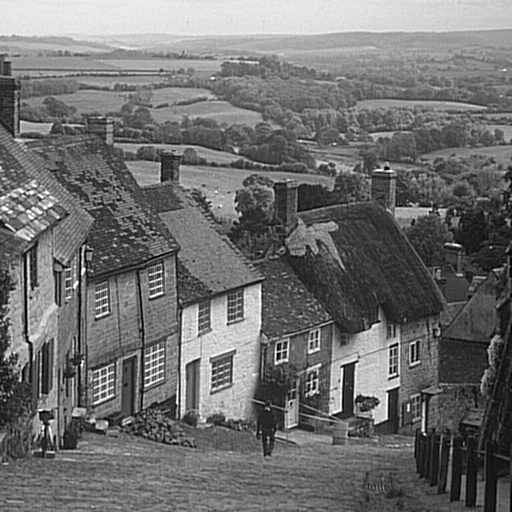
\includegraphics[width=0.9\textwidth]{resultados/city_h10.png}
        \caption{Convolução com $h_{10}$ (\ref{fig:h10}).}
    \end{subfigure}

    \caption{??}
    % \label{fig:blur}
\end{figure}
